\section{Interfejs użytkownika (Zofia Sosińska)}\label{c:elem_ui}

Dopuszczalnym założeniem przy tworzeniu gier komputerowych jest, że postać gracza ma jakąś wiedzę o świecie, w którym się znajduje oraz
poziom inteligencji i umiejętności, które pozwalają jej przeanalizować konkretną sytuację i wyciągnąć wnioski. Skoro więc te informacje są w zasięgu możliwości wnioskowania postaci, gra ma prawo wyświetlić je użytkownikowi. 

Takie graficzne przedstawienie najważniejszych danych z otoczenia gracza nazywamy interfejsem użytkownika UI (ang. \textit{user interface}). Narzędziami odzwierciedlania informacji
w czytelny i przystępny sposób mogą być takie elementy jak obrazki, teksty, czy wskaźniki. Takie zabiegi estetyczne sprawiają, że przetwarzamy suche dane
na interesujące informacje. "Interfejs użytkownika w grze ma służyć zarówno rozrywce, jak i ułatwieniu dostępu."\cite{projektowanie_podstawy}
Dzięki UI możliwy jest wgląd w aktualny stan wiedzy postaci gracza, a tym samym lepsze
zrozumienie otoczenia. Wymagające podkreślenia jest, że “[...] na stopień zaangażowania gracza na poziomie świata gry duży wpływ ma interfejs, którym się posługuje. Mówiąc najprościej:
gracz, który rozpoczyna grę, zanim dozna poczucia integracji ze sterowaną przez siebie postacią, musi - używając stwierdzenia Aarsetha - spełnić oczekiwania interfejsu.”\cite{olbrzymwcieniu}

Jednym z kluczowych problemów przy projektowaniu elementów interfejsu użytkownika jest odpowiednie wybranie miejsca na ekranie. Konieczne jest zwrócenie uwagi na takie 
problemy, jak  rozmiar, rola, priorytet dostarczenia informacji, częstość i długość występowania oraz częstotliwość zmiany zawartości.
Inną ważną cechą dobrze zaprojektowanego interfejsu użytkownika jest zbalansowanie między pokazaniem jak największej liczby kluczowych informacji, 
jednocześnie odkrywając je tak, aby nie przytłaczały gracza i nie zaciemniały przekazu.
Często dane segreguje się według ich tematyki, ale czasem właściwsze może okazać się zgrupowanie ich 
względem tego, jak często gracz będzie ich potrzebował. Jeśli są to informacje niezbędne do zrozumienia aktualnego 
stanu świata gry, wartościowe może być pokazanie ich obok siebie. Wszystkie te czynniki mają za zadanie ułatwić użytkownikowi
wyszukanie informacji. "Gdy czegoś szukamy, nasze spojrzenie jest prowadzone przez zainteresowanie wizualne.
Trudne do wyobrażenia jest jak zainteresowanie wizualne działa; jakie rodzaje procesów działają w mózgu kiedy decydujemy się spojrzeć i na
którym obszarze po chwili skupimy wzrok."\cite{user_interfaces} Przy projektowaniu interfejsu użytkownika kluczowe jest rozplanowanie
tego, które elementy, w jaki sposób i jak bardzo będą przykuwać uwagę użytkownika. Przy elementach, których treść użytkownik może przeglądać
lub zmieniać najważniejszą cechą jest łatwość i przyjemność obsługi. "[...] prawdopodobnie nie ma innego wyjścia, niż projektowanie programów tak,
 aby nie potrzebowały instrukcji obsługi."\cite{ui_for_programmers} Inaczej będzie on gracza męczyć i rozpraszać.

Przykładem zaprojektowania zbalansowanego elementu interfejsu użytkownika jest rozwiązanie gry Warcraft III: Reign of Chaos studia Blizzard Entertainment.
Zgrupowała ona najbardziej podstawowe informacje o świecie gry i skupiła te dane w cienkim pasku na samej górze ekranu. 
Skład elementów tej części interfejsu użytkownika jest niezmienny: pola otwierające zakładki, pora dnia oraz trzy wskaźniki zasobów. Pasek jest widoczny
podczas całej rozgrywki, niezależnie od wykonywanych czynności. W tym statycznie zakotwiczonym na górze ekranu elemencie, dynamicznie
zmieniają się jedynie ciągle aktualizowane informacje. Odpowiednio podmieniana jest tekstura pory dnia, zmieniająca się ze Słońca
na Księżyc oraz stan zasobów, zależnie od wydania, czy pozyskania.

\begin{figure}[htbp]
    \centering
    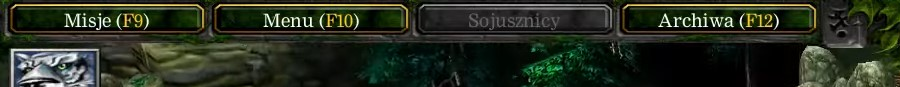
\includegraphics[width=1.0\textwidth]{images/ui/warcraft3_gorny_pasek_lewy.png}
    \caption{Lewa część paska z informacjami w grze Warcraft 3.}\label{fig:Warcraft3}
\end{figure}

\begin{figure}[htbp]
    \centering
    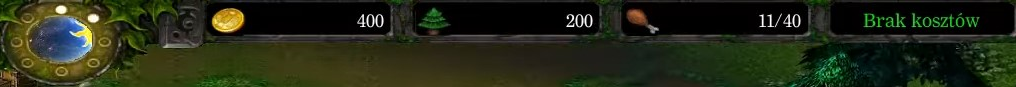
\includegraphics[width=1.0\textwidth]{images/ui/warcraft3_gorny_pasek_prawy.png}
    \caption{Prawa część paska z informacjami w grze Warcraft 3.}\label{fig:Warcraft3}
\end{figure}

Innym przykładem dobrze zaplanowanego UI jest przedstawienie dostępnych do zbudowania pułapek w grze
Orcs must die! studia Robot Entertainment. Zadaniem gracza jest wcielenie się w jednego z Wojennych Magów i mordowanie nadciągających grup orków za pomocą różnorodnych broni
i mechanizmów, które może postawić. Sam zakup mechanizmów jest sytuacją epizodyczną, dlatego grafiki pojawiają się, gdy gra jest w trybie stawiania budynków, 
i znikają poza nim. Rozwiązanie sprawia, że użytkownik nie jest rozpraszany przez niepotrzebny interfejs, gdy odpiera natarcie przeciwników. Zadbano także o 
optymalne umiejscowienie. Grafiki pojawiają się na dole ekranu tak, aby nie zasłaniać potencjalnego miejsca do postawienia budowli. Są to miniatury pułapek razem z 
ich ceną.

\begin{figure}[h!tbp]
    \centering
    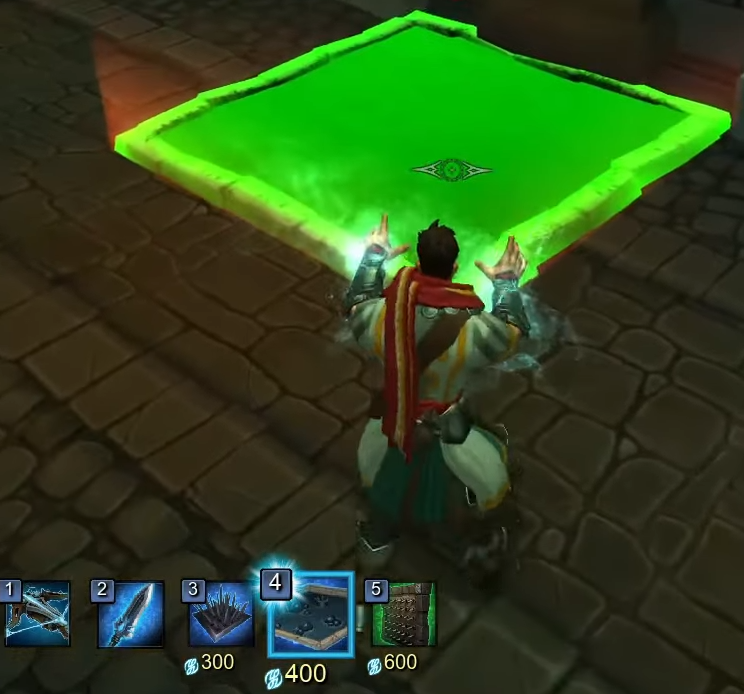
\includegraphics[width=0.9\textwidth]{images/ui/buoildingsOrcs.png}
    \caption{Wyświetlenie dostępnych pułapek w Orcs must die!}\label{fig:Orcs}
\end{figure}